\documentclass{article}
\usepackage[utf8]{inputenc}
\usepackage[spanish]{babel}
\usepackage{graphicx, graphics, float, fancyhdr, titling}
\usepackage{listings, subcaption}
\usepackage[a4paper, total={6in, 9.5in}]{geometry}
\usepackage{hyperref}

\setcounter{secnumdepth}{-2}


\renewcommand{\footrulewidth}{0.4pt}
\title{

\includegraphics[width=1.75in]{imagenes/UGR-Logo.png} \\
\vspace*{1in}
\textbf{Práctica 2, Sesión 2} \\
Seguridad en Sistemas Operativos \\
\vspace*{0.5in}}
\author{Andrés Merlo Trujillo \\
\vspace*{0.5in} \\
E.T.S. de Ingenierías Informática y de Telecomunicación \\
\textbf{Universidad de Granada}} \date{\today}
%\date{}
\hypersetup{
    colorlinks=true,
    linkcolor=black,
}

\renewcommand\maketitlehooka{\null\mbox{}\vfill}
\renewcommand\maketitlehookd{\vfill\null}

\begin{document}
\begin{titlingpage}
    \maketitle
\end{titlingpage}

\tableofcontents

\newpage

\pagestyle{fancy}
\fancyhead[L]{Andrés Merlo Trujillo}
\fancyhead[R]{Seguridad en Sistemas Operativos}

%\addcontentsline{toc}{section}{Ejercicio 1}
%\section{Ejercicio 1}
%\begin{figure}[H]
%    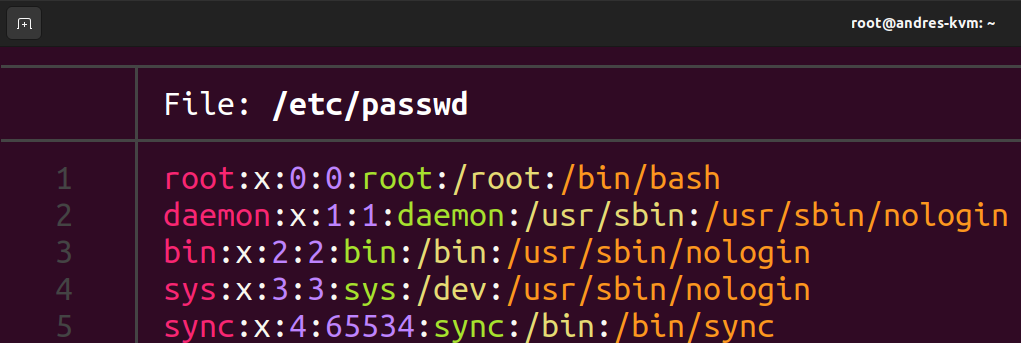
\includegraphics[width=\textwidth]{imagenes/passwdfile.png}
%    \caption{Ejemplo de entradas en el archivo.}
%\end{figure}

\section{Ejercicio 1}

\textbf{Enunciado: }``Para el sistema que utilizas, indica la arquitectura, distribución y compilador que utilizas e indica que protecciones se utilizan de cara a proteger un binario ELF.''

\bigskip

Para obtener la arquitectura de la CPU, voy a utilizar la orden \verb|lscpu|.

%foto de lscpu
\begin{figure}[H]
    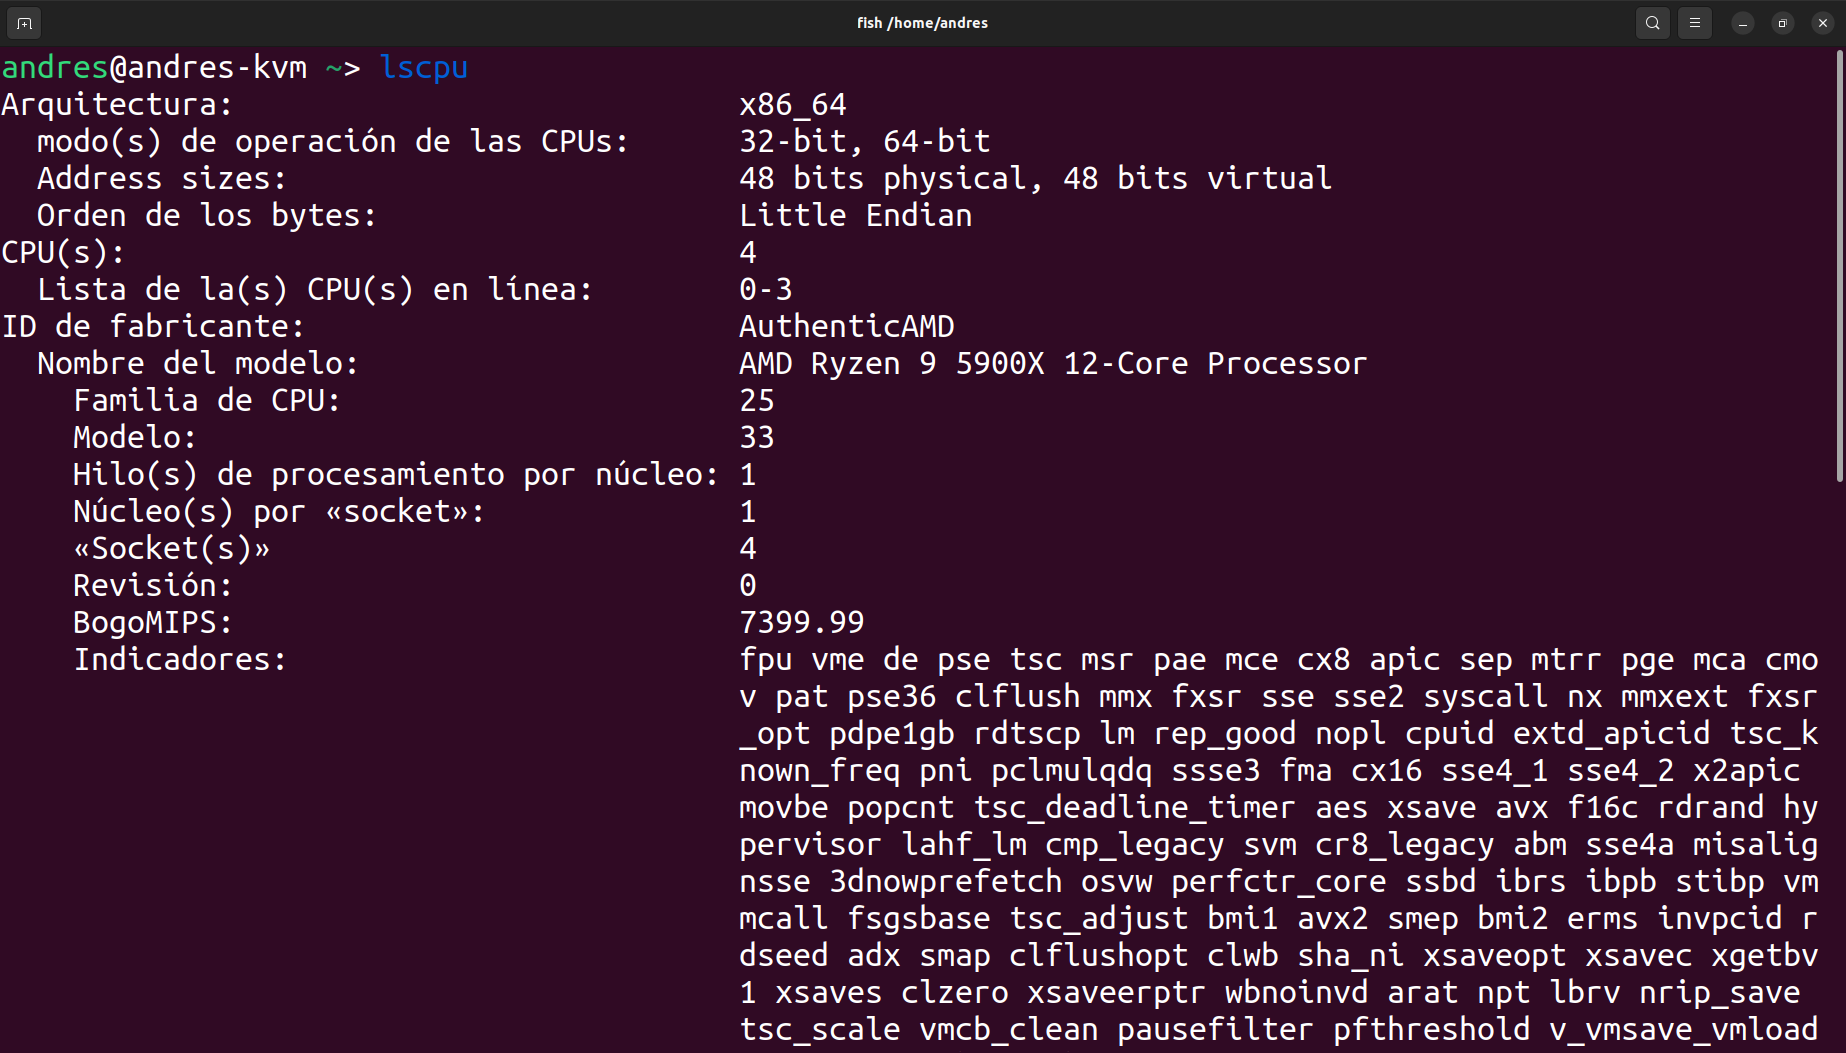
\includegraphics[width=\textwidth]{imagenes/Captura desde 2022-11-23 10-33-11.png}
    \caption{Salida del comando.}
\end{figure}

\bigskip

Para saber la distribución, hay dos formas: la primera depende del entorno de escritorios (DE), pero como en mi caso es GNOME 42 se puede hacer yendo a Configuración y Acerca de:

%foto de esta pantalla
\begin{figure}[H]
    \centering
    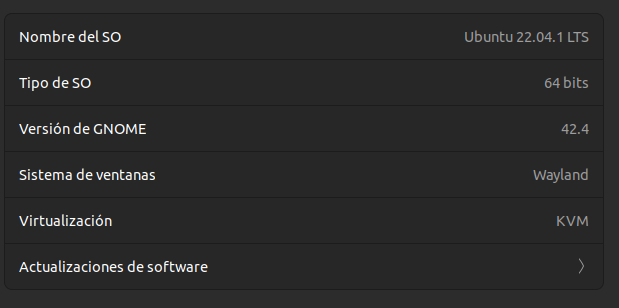
\includegraphics[width=0.7\textwidth]{imagenes/Captura desde 2022-11-23 10-37-46.png}
    \caption{Distribución utilizada mediante los ajustes de GNOME.}
\end{figure}

\bigskip

La segunda opción es usando el comando \verb|lsb_release -a|, que indica por terminal la misma información:

%foto de la salida del comando
\begin{figure}[H]
    \centering
    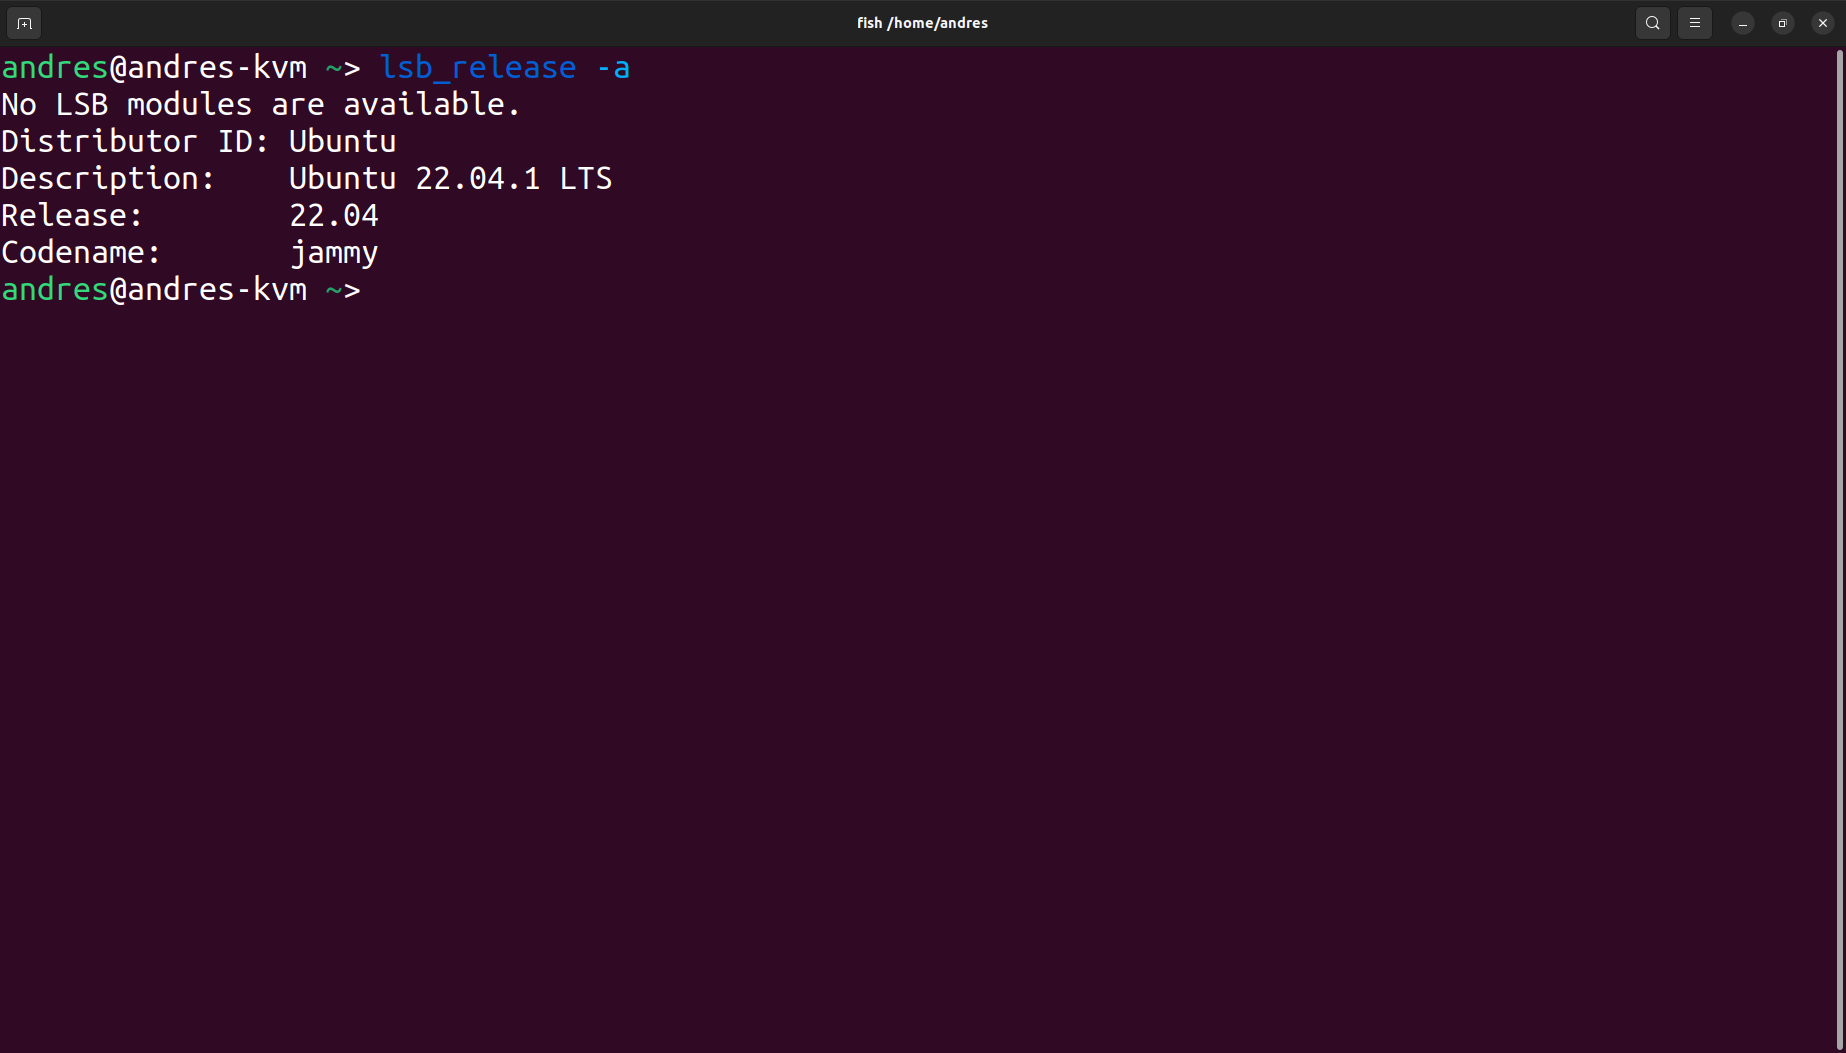
\includegraphics[width=0.6\textwidth]{imagenes/Captura desde 2022-11-23 10-38-58.png}
    \caption{Distribución utilizada mediante línea de comandos.}
\end{figure}

\newpage

Ahora, para obtener la versión del compilador, se utiliza el comando \verb|gcc --version|:

%foto de la version de gcc
\begin{figure}[H]
    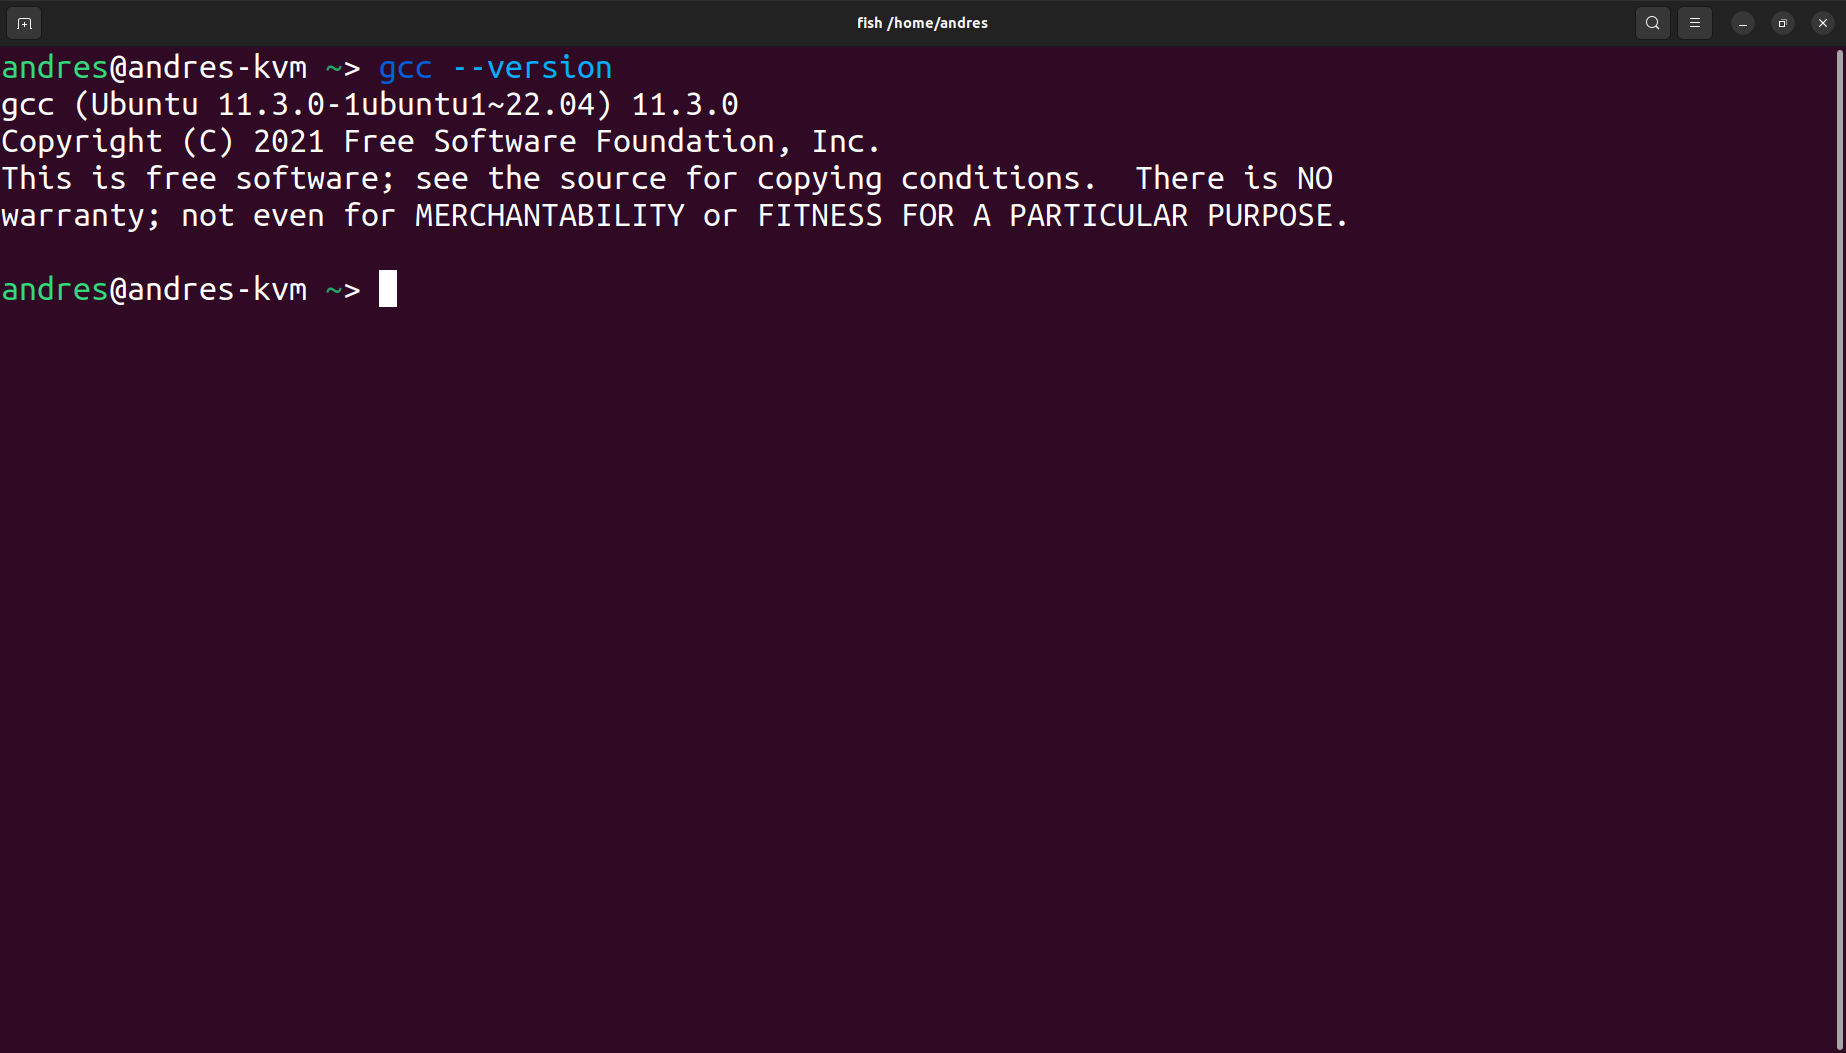
\includegraphics[width=\textwidth]{imagenes/Captura desde 2022-11-23 10-39-52.png}
\end{figure}


Ahora bien, los mecanismos para proteger los binarios ELF son diversos y se encuentran implementados en el kernel y en el compilador. Las protecciones del kernel son las siguientes:

\begin{itemize}
    \item \textbf{ASLR (Aleatorización de la disposición del espacio de direcciones)}: Tiene como objetivo evitar la ejecución de código malicioso como puede ser \textit{shellcode} debido a una función del programa vulnerable. ASLR permite aleatorizar en cada ejecución del programa las distintas partes del mismo, como el código del programa, bibliotecas, etc. Esto hace que sea más difícil que un atacante sepa donde se encuentra la parte vulnerable al ser en cada ejecución distinta.
\end{itemize}

\bigskip

Mientras que para la parte del compilador hay los siguientes mecanismos:

\begin{itemize}
    \item \textbf{Protección de pila ejecutable}
    \item \textbf{Protección de rotura de pila}: Mediante el uso de la macro \verb|FORTIFY_SOURCE|, el compilador dará warnings en las secciones de código que potencialmente puedan producir un buffer overflow. Además, en tiempo de ejecución si detecta un buffer overflow aborta el programa y muestra un trace con toda la información en el momento del fallo.
    \item \textbf{Ejecutables independientes de la posición (PIE)}: Mediante la opción del compilador \verb|-pie| se produce un ejecutable independiente de la posición, esto quiere decir que las distintas partes del programa van a tener un offset para que no se encuentren siempre en una dirección fija.
    \item \textbf{Fuente fortificada}
    \item \textbf{Protector de pila}: Mediante la opción del compilador \verb|-fstack-protector| que habilita la protección de la pila. Hace uso de la técnica ``Stack Canary'', que es un valor que se le asigna a cada función al principio y que al final de la misma se espera que sea igual, si se ha producido un bug o un ataque el programa aborta al ser el valor distinto y se impide el potencial ataque.
\end{itemize}

\newpage

\section{Ejercicio 2}

\textbf{Enunciado: }``Podemos mejorar el siguiente virus:''
\subsection{Apartado A}

\textbf{Enunciado: }``Escribiendo un mejor escaner/limpiador para él.''

\bigskip

Para que el virus funcione, es necesario modificar el archivo \textit{elfvirus.c} y modificar las llamadas a la función \verb|searchForELF| para que use la ruta que he especificado.

%foto de eso
\begin{figure}[H]
    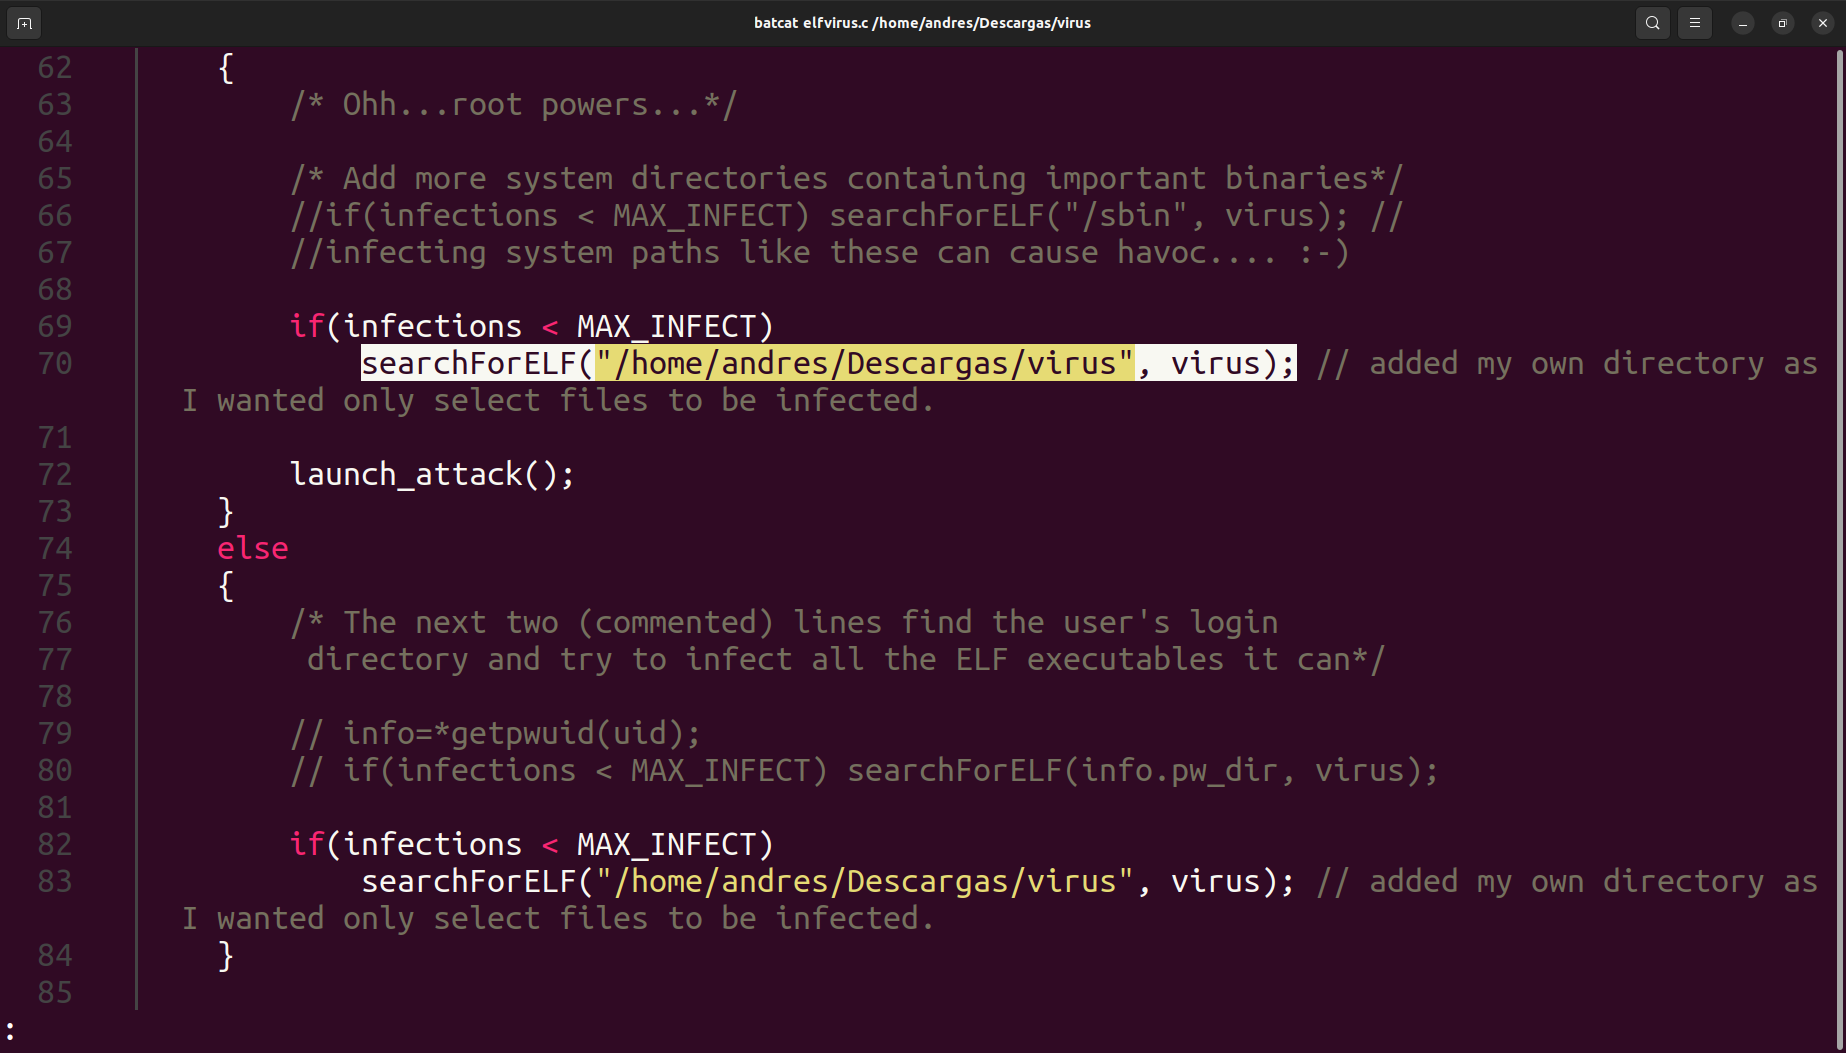
\includegraphics[width=\textwidth]{imagenes/Captura desde 2022-11-25 17-29-47.png}
    \caption{Modificación del directorio al que afecta el virus.}
\end{figure}


A continuación, es necesario compilar el programa y con la orden \verb|ls -l| se obtiene el tamaño del virus:

%foto del comando
\begin{figure}[H]
    \centering
    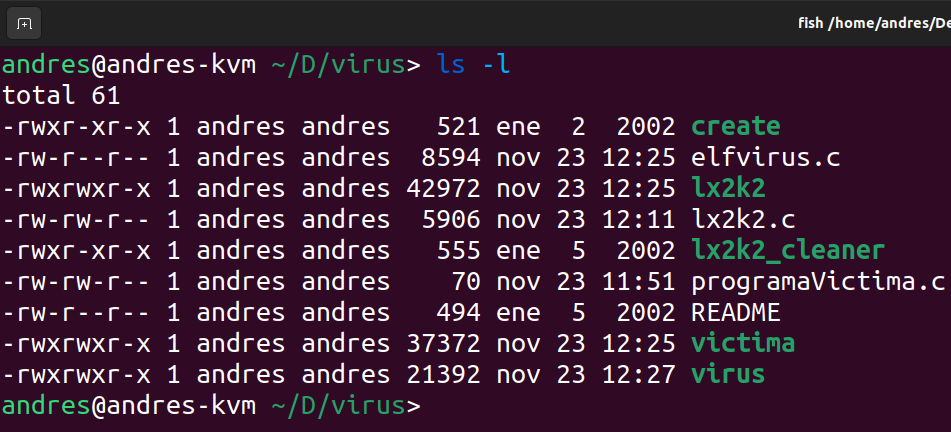
\includegraphics[width=0.7\textwidth]{imagenes/Captura desde 2022-11-23 12-28-06.png}
    \caption{El ejecutable se llama \texttt{virus}, y como se puede ver tiene un tamaño de \textbf{21932}.}
\end{figure}

\newpage

Por tanto, en el \verb|#define VIRUS_SIZE| se pone ese tamaño:

%foto del cambio
\begin{figure}[H]
    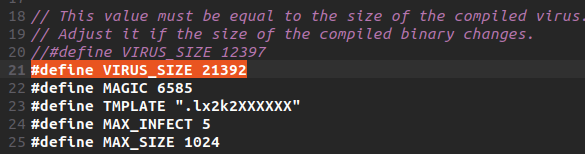
\includegraphics[width=\textwidth]{imagenes/Captura desde 2022-11-23 12-29-27.png}
    \caption{Cambio del tamaño del ejecutable del virus.}
\end{figure}

\bigskip

Se compila y ahora al ejecutar el virus infectado aparece lo siguiente:

%foto de la salida del virus
\begin{figure}[H]
    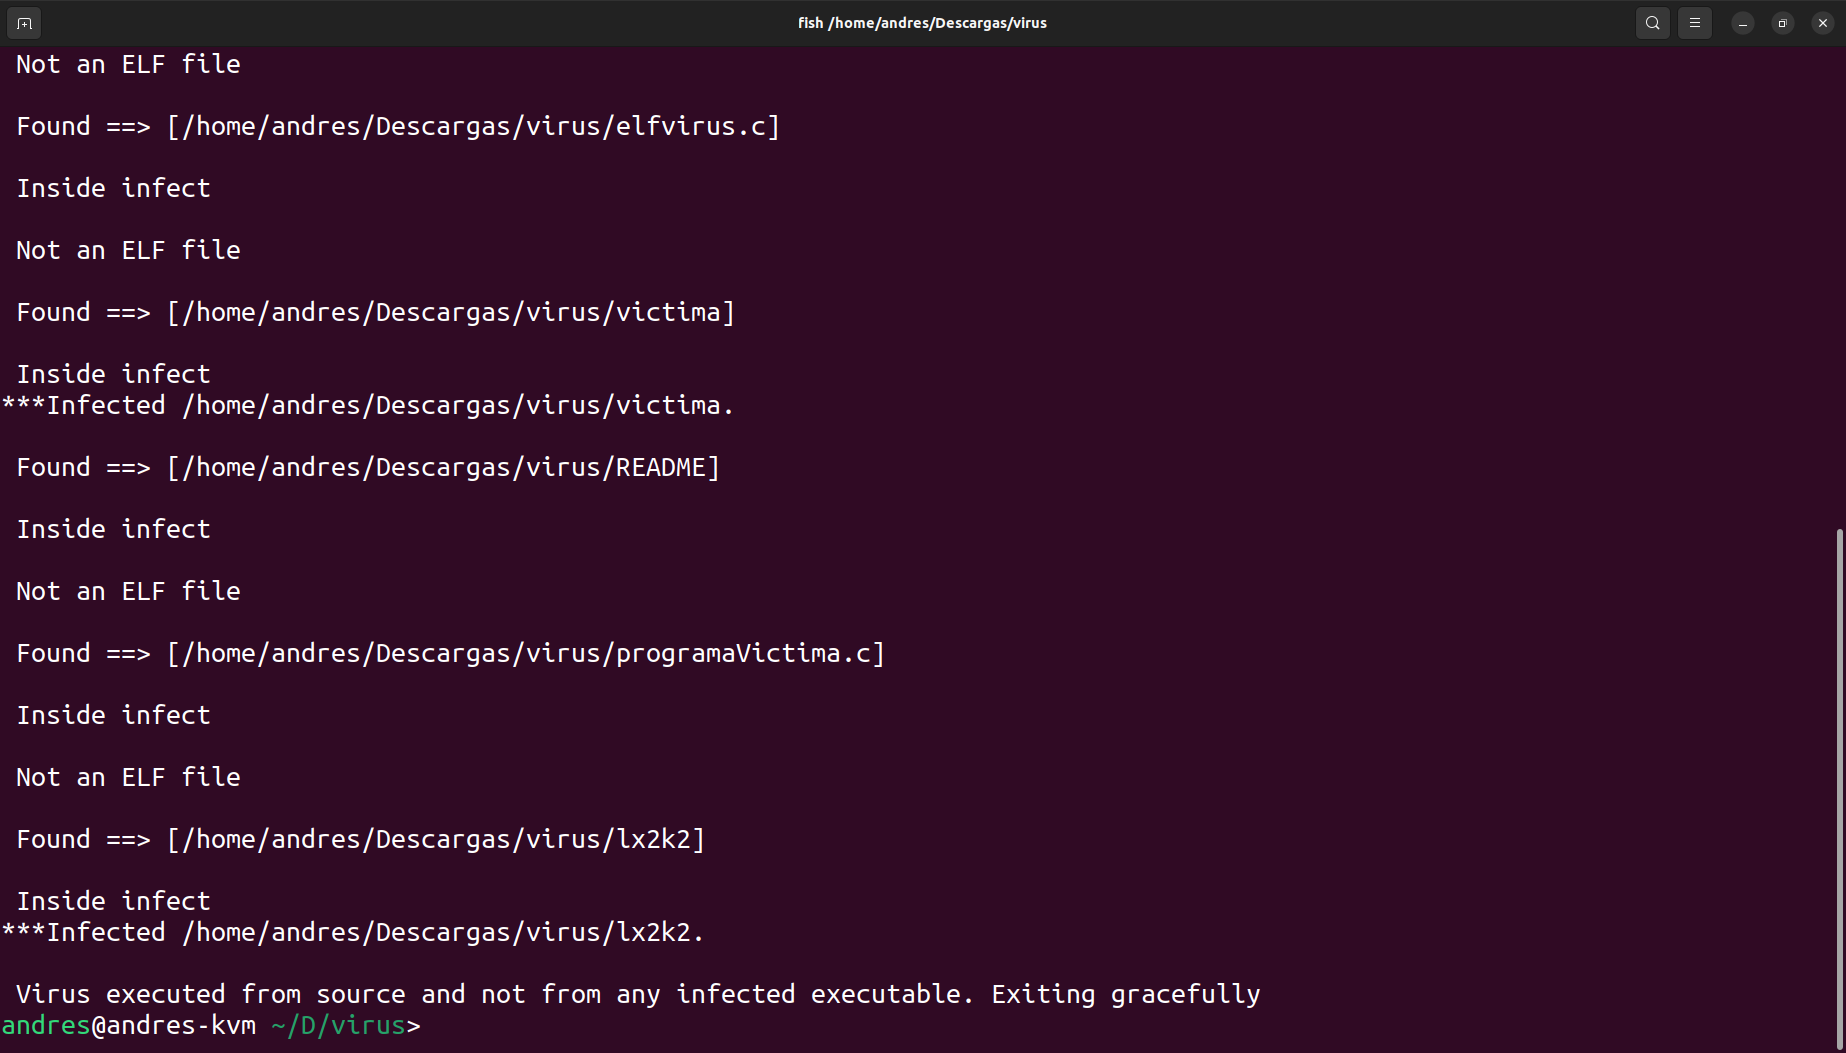
\includegraphics[width=\textwidth]{imagenes/Captura desde 2022-11-23 12-32-53.png}
    \caption{Salida de la ejecución del virus.}
\end{figure}

Como se puede ver ha infectado el programa \textit{victima}, que es un Hola Mundo escrito en C.

\newpage

Y si ahora ejecuto \textit{victima}, aparece lo siguiente:

%foto de la ejecucion de victima
\begin{figure}[H]
    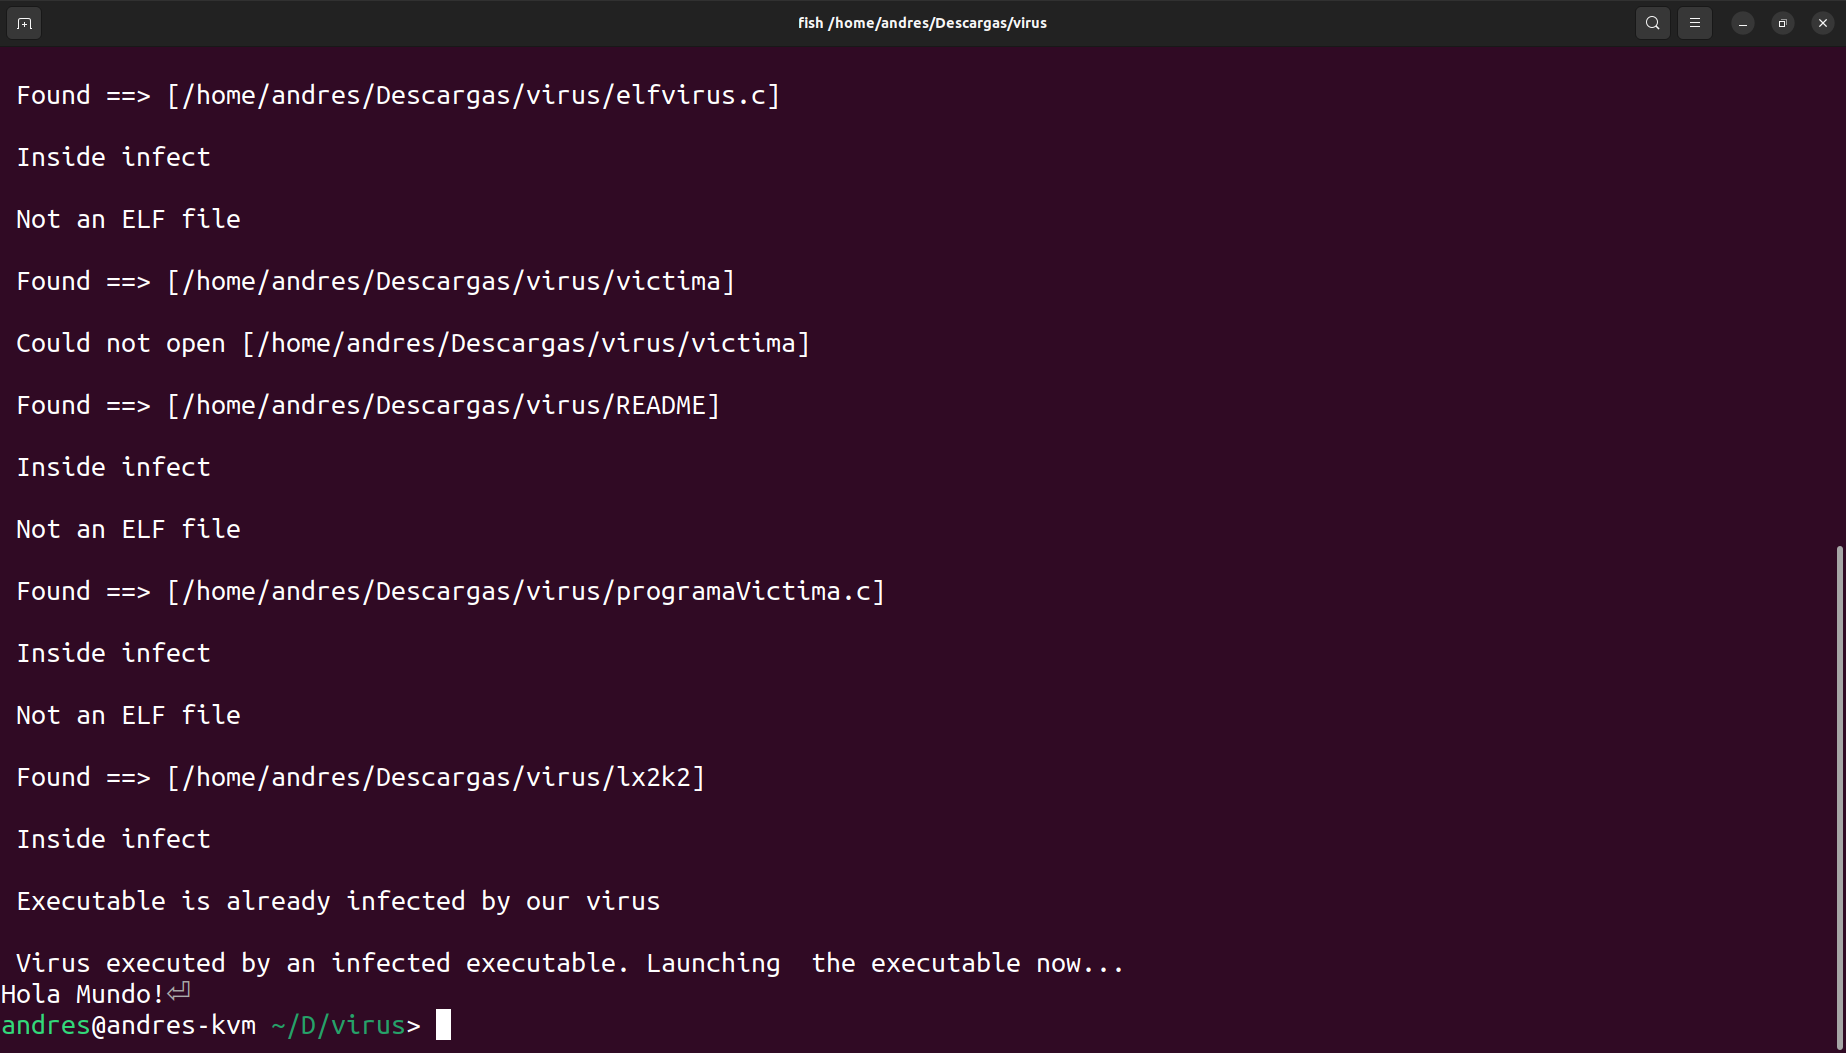
\includegraphics[width=\textwidth]{imagenes/victimaInfectada/Captura desde 2022-11-23 12-33-29.png}
    \caption{Se ve que primero se ejecuta el virus y después el contenido del ejecutable original.}
\end{figure}

Como se puede observar, este programa está infectado, y si lo pusiéramos en otro directorio infectaría a los otros. No obstante, esto no es posible porque gracias a la función \verb|searchForELF| se le ha restringido el acceso a solo la carpeta del virus, pero puede tener el potencial de hacer daño.

\bigskip

El script del limpiador tenía ciertos fallos que el intérprete detectaba, haciendo que no funcionase. Lo he arreglado haciendo las siguientes modificaciones: 

%foto del script limpiador
\begin{figure}[H]
    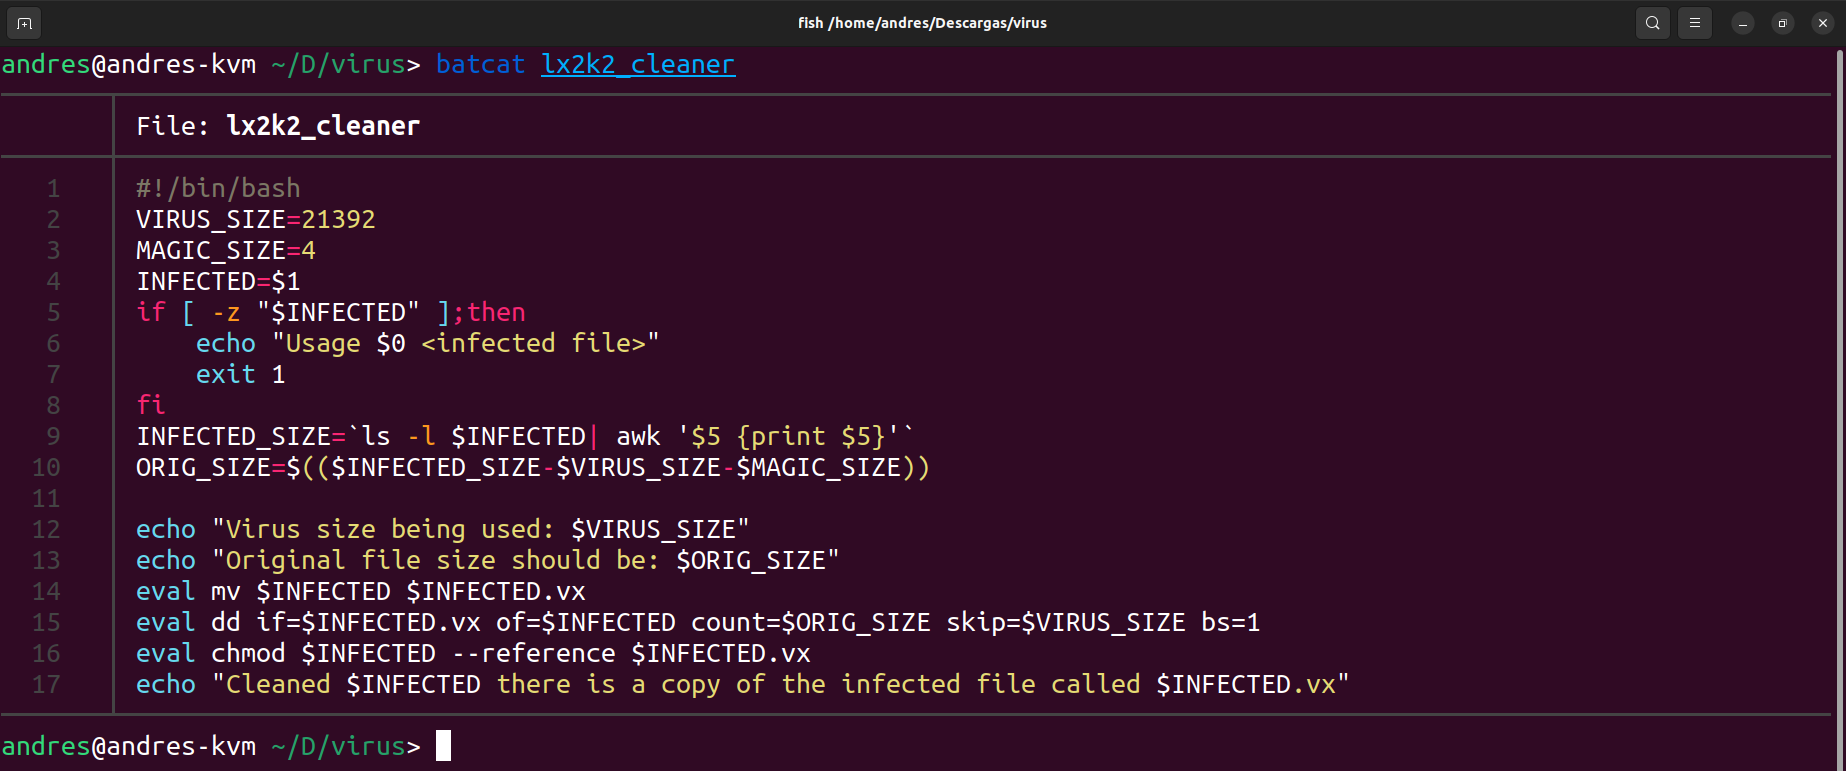
\includegraphics[width=\textwidth]{imagenes/Captura desde 2022-11-23 12-44-29.png}
    \caption{Se puede ver que ahora uso bash, he cambiado el tamaño del virus, he eliminado el \texttt{let} de \texttt{ORIG\_SIZE} y he hecho que haga bien la cuenta esta misma variable usando \texttt{\$(())} de bash.}
\end{figure}

\newpage

Después de estos arreglos, al ejecutarlo aparece lo siguiente:

%foto de la salida
\begin{figure}[H]
    \centering
    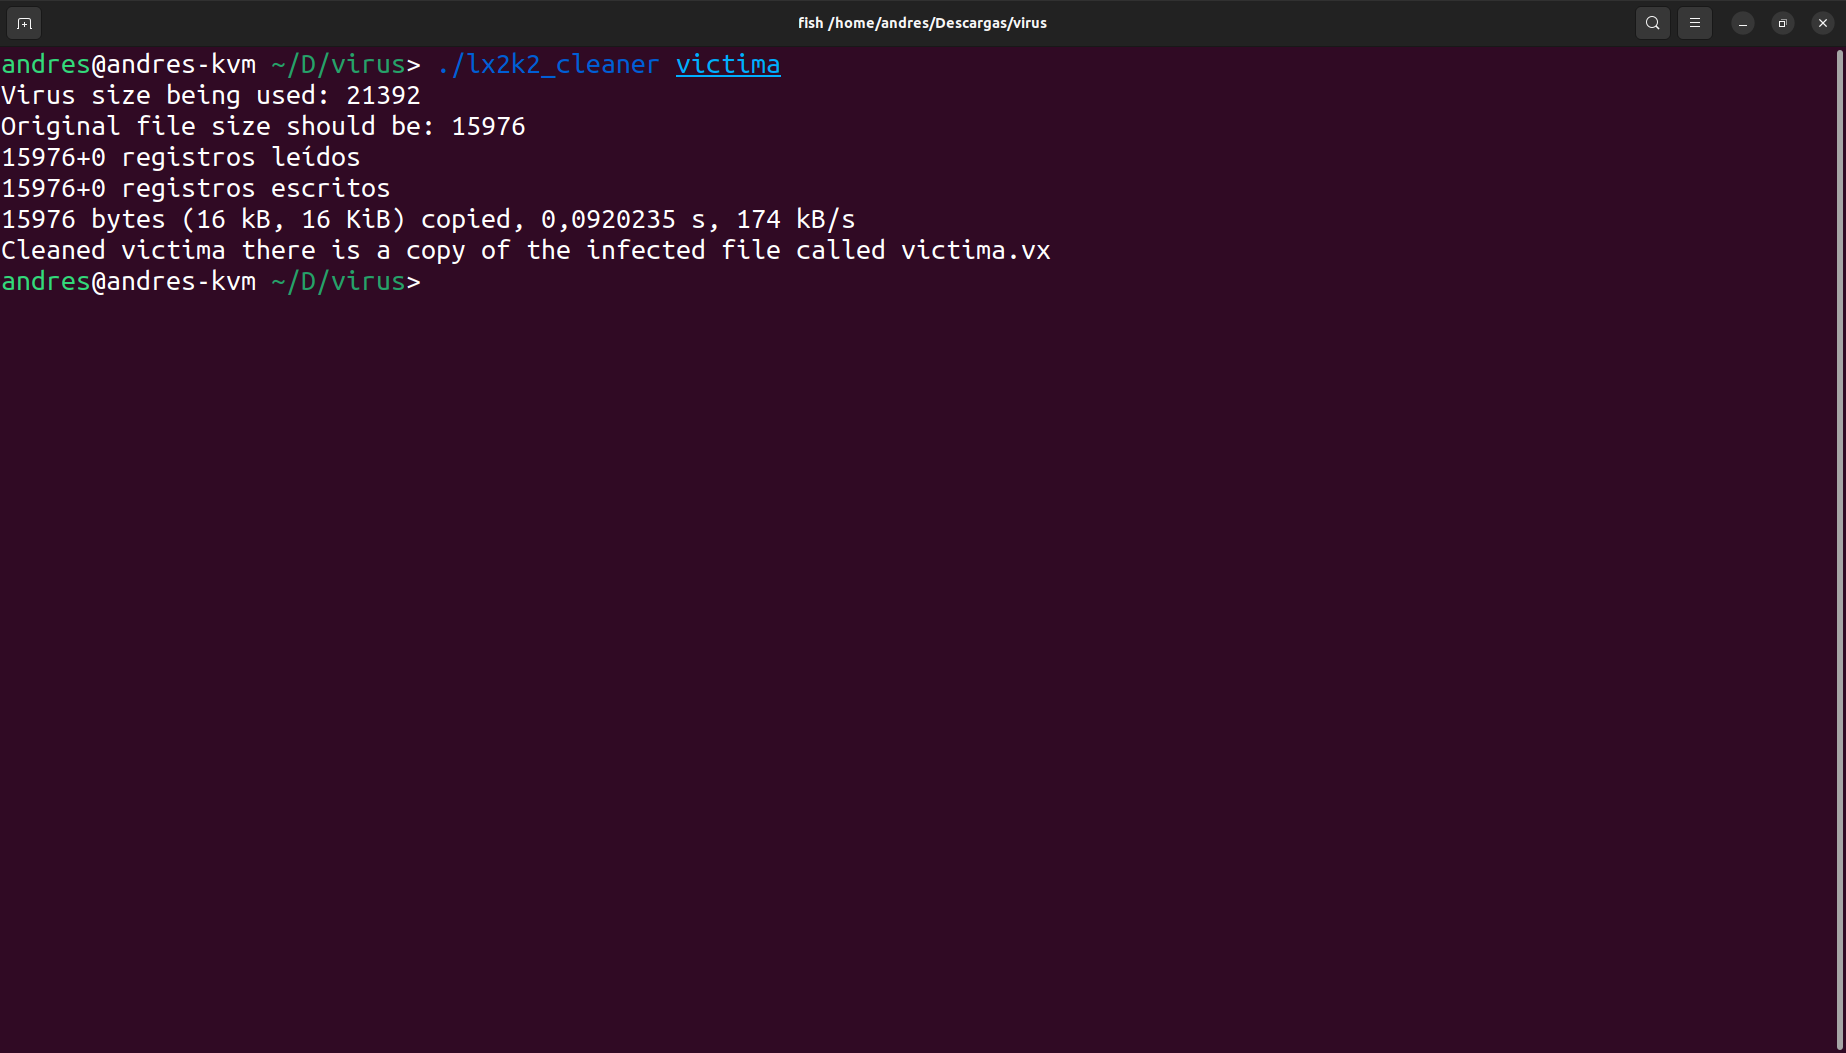
\includegraphics[width=0.8\textwidth]{imagenes/Captura desde 2022-11-23 12-45-50.png}
\end{figure}

\bigskip

Y ahora al ejecutar el ejecutable ``saneado'', aparece la salida correctamente sin ejecutar el virus.

\bigskip

El limpiador se podría mejorar haciendo que en vez de tener que ir ejecutable a ejecutable uno a uno a mano, se pueda pasar un directorio y de manera recursiva vaya limpiando los ejecutables infectados. Para ello, haría falta que el script hiciese una comprobación de si existe el virus en el ejecutable, ya que siempre intenta eliminar los primeros 21932 Bytes del programa, que es donde reside el virus.

\subsection{Apartado B}

\textbf{Enunciado: }``Añadir \verb|#ifdef| para comprobar la arquitectura de forma que cambie de forma automática el valor \verb|EM_386| en tiempo de compilación para adaptarlo al sistema donde estemos.''

\bigskip

Usando un editor de texto avanzado o un IDE como Visual Studio Code, se puede ver que la estructura de datos \verb|Elf32_Ehdr| contiene las siguientes arquitecturas (no son todas) en el archivo \verb|elf.h|:

%foto de las arquitecturas
\begin{figure}[H]
    \centering
    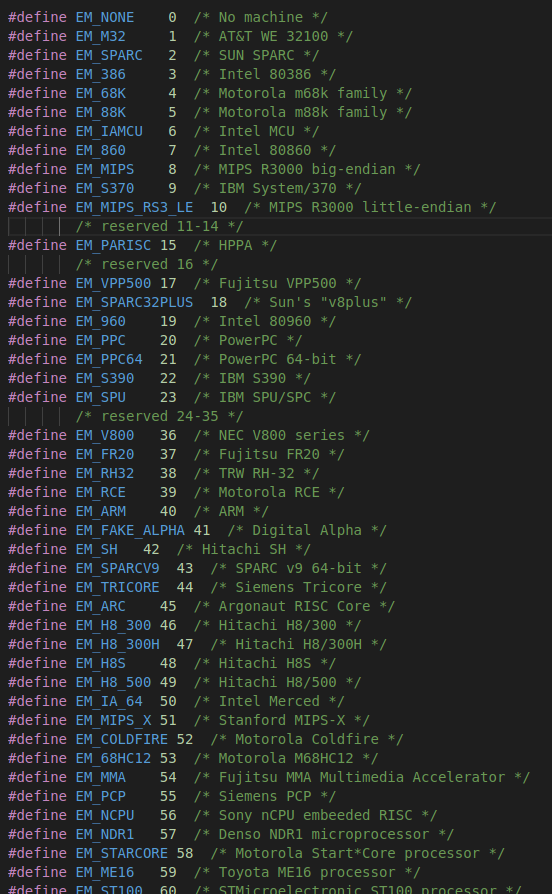
\includegraphics[width=0.45\textwidth]{imagenes/Captura desde 2022-11-23 13-07-09.png}
    \caption{Alguna de las arquitecturas disponibles.}
\end{figure}

Y la lista continúa hacia abajo, por lo que solo voy a realizar la comprobación de si es x86, x86\_64, ARM, ARM64, PowerPC y IA64 (Itanium). 

\newpage

Para realizarlo, es necesario usar macros que el compilador \verb|gcc| posee, la lista se encuentra en: \url{https://sourceforge.net/p/predef/wiki/Architectures/}.

\bigskip

Por tanto, el código del virus quedaría así:

%foto del trozo de codigo modificado
\begin{figure}[H]
    \centering
    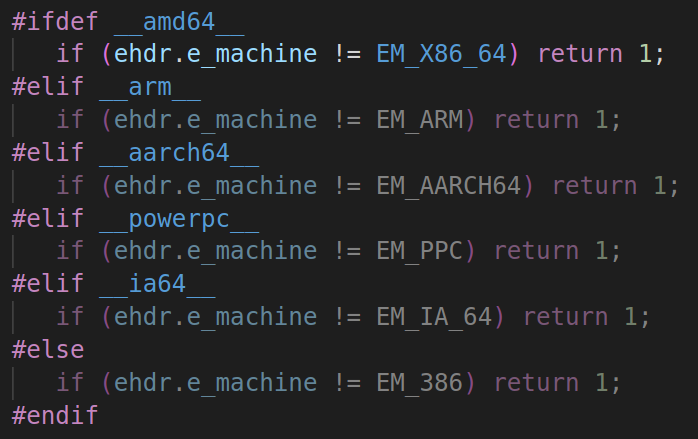
\includegraphics[width=0.7\textwidth]{imagenes/Captura desde 2022-11-25 17-21-11.png}
    \caption{Modificación del programa \texttt{lx2k2.c} para cambiar el código en tiempo de compilación.}
\end{figure}



\end{document}
